\documentclass[usenatbib]{tjaa}

\usepackage[utf8]{inputenc}

\usepackage{lipsum}
 
\newsavebox\verbbox

\title[Short Title max 45 chars]{Leverage data fusion from s1-s2 to enable\newline  
fast and accurate land cover classification}

% NOTES (authors):
% 1) For single author don't number single affiliation addreess.
% 2) If you need two or more lines of authors, use \newauthor (see below usage)
% 3) ORCID is required for ALL authors
% 4) Short author should be either A.U. Thor et.al -or- A. U. Thor
% 5) Depending on the language \others will be either "et al." or "v.ark."
\author[F. Author \others]{%
Crampe Marc\autid{1}{0000-0000-0000-0000}\thanks{crampemarc@gmail.com},
Picard Emilio\autid{2}{0000-0000-0000-0000}\thanks{emilio.picard@free.fr},
\\
% NOTES (List of institutions):
% 1) Don't put \\ at the last institution
\adrid{1}IPSA, Department of Engeneering, 75000, France\\
\adrid{2}ENS Paris Saclay, Department of Mathematics, 91000, France\\
}%%%%TJAA-OZEL:AUTHOR%
% These dates and numbers will be filled out by the publisher
\date{Accepted: XXX. Revised: YYY. Received: ZZZ.}
%
\renewcommand{\pubyear}{0000}
\renewcommand{\volume}{0}
\renewcommand{\issue}{0}

% NOTES (language):
% 1) Default language of TJAA is ENGLISH.
% 2a) If your manuscript is in ENGLISH then leave both commands as commented
%\ENlang
% 2b) If your manuscript is in TURKISH then uncomment only below command
%\TRlang

\begin{document}
% Don't change these 3 lines
\label{firstpage}
\pagerange{\pageref{firstpage}--\pageref{lastpage}}
\maketitle{M00-0000}

\begin{abstract}
  Urban areas face unique challenges in monitoring and managing land cover changes,
  particularly due to cloud cover that a9ects optical imagery. This study presents an innovative
  approach to urban land cover classification by fusing \texttt{Sentinel-1} Synthetic Aperture Radar ($SAR$)
  data with \texttt{Sentinel-2} optical data. We aim to develop an automated algorithm capable of
  providing monthly monitoring of urban land cover changes, enhancing classification accuracy
  and o9ering critical insights into urban growth and environmental resilience.
  \\
  Utilizing a combination of $4$ images from \texttt{Sentinel-1} (VV, VH, VV/VH) and $5$ key spectral indices
  derived from \texttt{Sentinel-2} (NDVI, SAVI, BAI, NDWI, and alternative BAI), we created a
  comprehensive merged dataset of $20$ bands. This dataset serves as the foundation for our
  classification models, including Support Vector Machines (SVM), K-Nearest Neighbors (KNN),
  Random Forest (RF), and Neural Networks (NN), which are evaluated for their performance in
  accurately classifying various urban features.
  \\
  Additionally, we explore Convolutional Neural Networks (CNN) and the \texttt{SAM2} model for
  advanced classification techniques. Our results demonstrate the potential of SAR and optical
  data fusion to overcome the limitations of cloud cover, providing a robust framework for
  automated urban land cover monitoring. This research contributes to a better understanding of
  urban dynamics and supports e9ective environmental management strategies. \cite{einstein1905}
\end{abstract} 

\begin{keywords}
data fusion -- machine learning -- geospatial
\end{keywords}

\section{Introduction}

\noindent
In recent years, approximately 90\% of the world's mapping data has been generated,
underscoring the critical importance of leveraging state-of-the-art technologies to create
accurate maps that reflect the real challenges facing our planet today. The rapid pace of
urbanization has transformed cities, leading to an urgent need for precise tools that can
monitor land cover evolution. By comprehensively understanding these changes, we can
identify detrimental impacts on the environment while also highlighting effective remediation
efforts, ultimately contributing to the development of greener, more sustainable urban
landscapes.
\\
\\
However, the utility of optical imagery, particularly from satellites like Sentinel-2, is often
compromised by cloud coverage, especially in tropical and coastal regions. This phenomenon
results in significant data gaps, which can severely limit the effectiveness of urban monitoring
tools. For instance, in Rouen, France, persistent cloud cover restricts the availability of usable
optical images to only ten per year, presenting a substantial challenge for consistent urban
analysis.
\\
\\
To address these limitations, this study focuses on the exploitation of classification models on
fused Sentinel-1 Synthetic Aperture Radar (SAR) and Sentinel-2 optical data. By employing
data fusion techniques to mitigate the impacts of cloud coverage, we aim to enable more
reliable monthly monitoring of urban land cover changes. The primary objective of this
research is to evaluate and compare various machine learning and deep learning models—
including Random Forest, Support Vector Machines (SVM), and Convolutional Neural
Networks (CNNs)—to identify the most effective methodologies for achieving accurate and
robust land cover classification in urban environments.
\begin{figure}
  \centering
  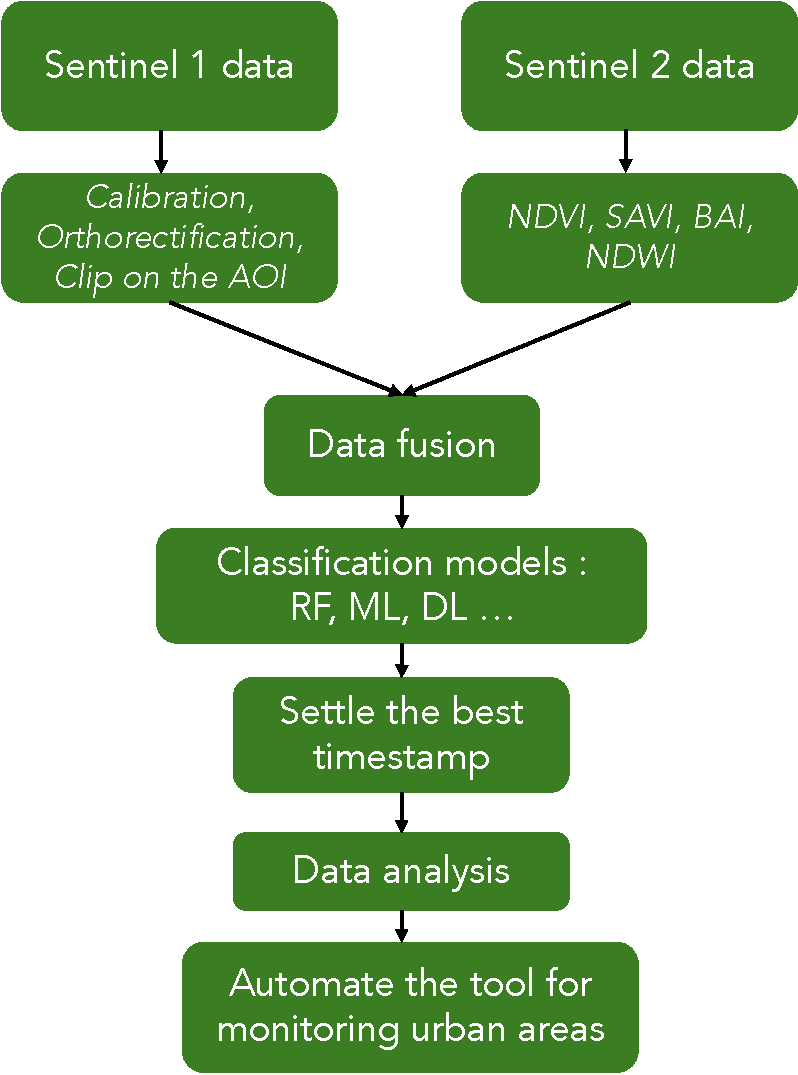
\includegraphics[width=.6\linewidth]{./figures/diagramme_sec1.pdf}
  \caption{Diagram of algorithm implementaion}
  \label{diagram-s1}
\end{figure}
\\
\\
Diagram \ref{diagram-s1} show the pipeline of our implementation for testing our method and
compare to the \textit{naive} ones.
\subsection*{Why Rouen?}
\noindent
Rouen, a historic city in northern France, presents a diverse urban landscape with a mixture of
commercial, residential, and industrial zones, as well as surrounding vegetation and water
bodies (the Seine River). Its coastal proximity also makes it a relevant choice for studying urban
resilience and environmental dynamics, as it faces potential impacts from coastal erosion and
urban expansion.

\subsection*{Urban Dynamics and Environmental Challenges}
\begin{itemize}
  \item Population: Approximately $111,000$ inhabitants in the city center, with a wider metropolitan
  area exceeding $500,000$ residents.
  \item Urban Challenges: Urban growth, environmental remediation e9orts, and flood management
  due to its proximity to the river and low-lying coastal areas.
  \item Environmental Focus: Monitoring urban development, green spaces, and remediation
  strategies aimed at reducing the environmental footprint of urban sprawl. 
\end{itemize}

\subsection*{Application of Data Fusion and Models}
\noindent
For this study, we applied the Sentinel-1 and Sentinel-2 data fusion approach to analyze the land
cover changes in Rouen. The various machine learning models (SVM, KNN, RF, NN, CNN, and
SAM2) were trained and tested on this region, allowing us to evaluate the accuracy and
robustness of each approach in distinguishing between urban features.
\\
\\
\noindent
We utilize data from both \textbf{Sentinel-1} (SAR) and \textbf{Sentinel-2} (optical) to overcome challenges like
cloud cover in urban land cover classification. \\
Sentinel-1 provides radar data (VV, VH, and VV/VH ratio) that is resistant to cloud cover, allowing
consistent monitoring of urban structures and vegetation. \\
Sentinel-2 supplies optical data, from which we calculate 4 key spectral indices specifically
designed to distinguish urban features:
\begin{itemize}
  \item \textbf{NDVI} (Normalized Difference Vegetation Index): highlights vegetation health
  \item \textbf{SAVI} (Soil Adjusted Vegetation Index): Adjusts for soil influence in areas with sparse vegetation
  \item \textbf{BAI} (Burned Area Index): Detects bare soil and sparse vegetation
  \item \textbf{NDWI} (Normalized Di9erence Water Index): Identifies water bodies and moisture
\end{itemize}
The use of these indices allows us to highlight specific features that are not visible to the naked
eye by combining di9erent spectral bands to extract precise information. For example, the NDVI,
which uses the red and near-infrared bands, detects vegetation health by distinguishing areas
with dense vegetation cover from those where vegetation is in decline. Similarly, the SAVI, a
modified version of NDVI that accounts for exposed soil, is crucial in environments with sparse
vegetation. The BAI, using blue and near-infrared bands, detects areas with bare soil or minimal
vegetation, often associated with phenomena like fires or erosion. Lastly, the NDWI, which
combines the green and near-infrared bands, identifies water bodies or moisture presence,
providing key information for assessing hydrology and flood risks.\\
\\
\noindent
When combined with Sentinel-1 radar data, which is resistant to cloud cover, these indices
enable more accurate and detailed analysis of urban land cover changes. This fusion of data
enhances our ability to monitor and predict environmental transformations in cities, improving
decision-making for urban planning and disaster mitigation.
\\
\\
\noindent
The final merged image consists of 20 bands:
\begin{itemize}
  \item Sentinel-1: 4 images × 3 bands (VV, VH, VV/VH)
  \item Sentinel-2: The 5 special indices plus the original B2, B3, B4, B8 bands 
\end{itemize}
All those different bands can be seen in figure \ref{20-bands}. Figure \ref{S1-S2-bands}
show the multispectral data visualization of S1 and S2. 
\begin{figure}
  \centering
  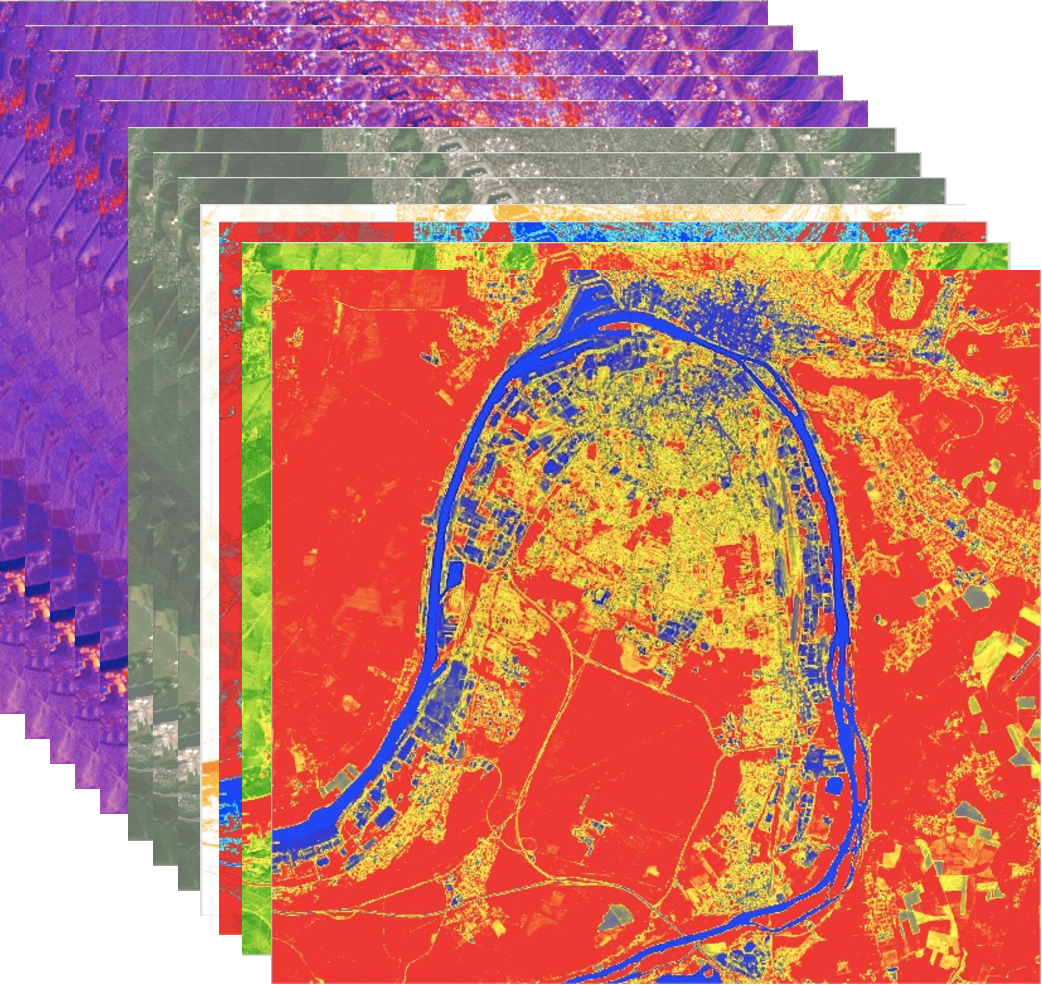
\includegraphics[width=.6\linewidth]{./figures/merged_images_sec2.pdf}
  \caption{Final merged image with the 20 different selected bands.}
  \label{20-bands}
\end{figure}
\begin{figure}
  \centering
  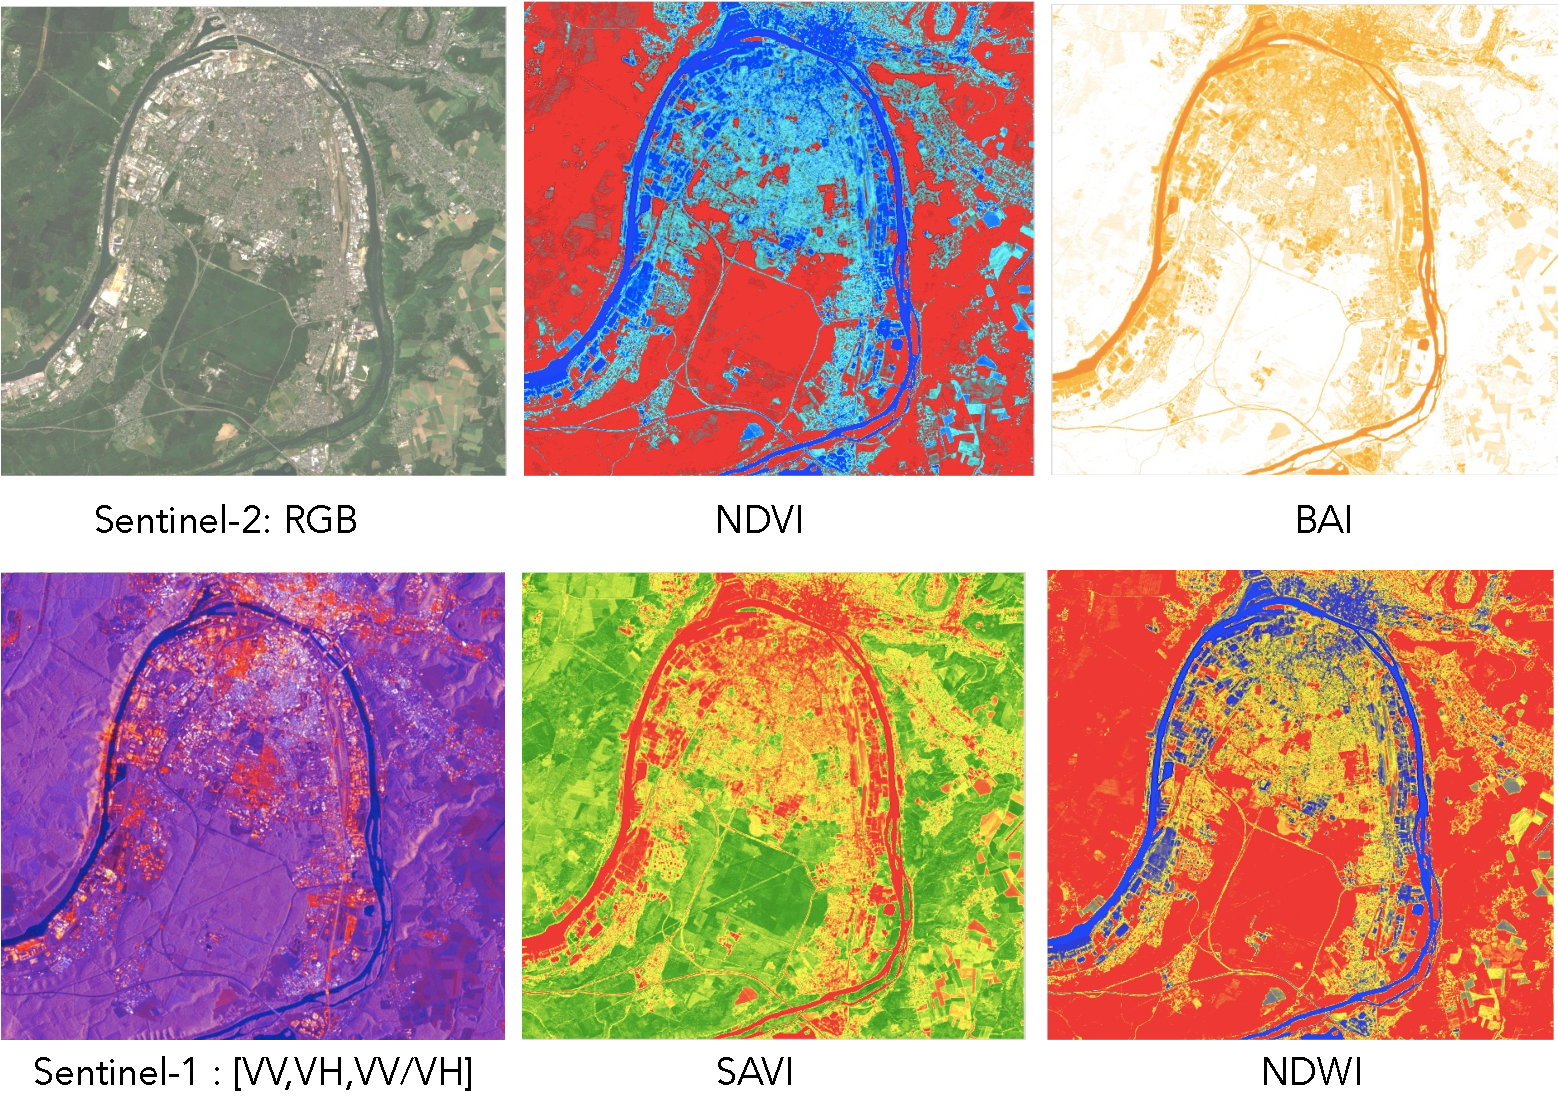
\includegraphics[width=.9\linewidth]{./figures/Image_index.pdf}
  \caption{Multispectral Data Visualization of Sentinel-1 and Sentinel-2.}
  \label{S1-S2-bands}
\end{figure}
\\
\\
The final merged image consists of 20 bands, formulated as follows:
\\
\\
\textbf{Merged Image} = \[VV_1, VV_2, VV_3, VV_4, VH_1, VH_2, VH_3, VH_4, VV/VH_1, VV/VH_2,
VV/VH_3, VV/VH_4, NDVI, SAVI, BAI, NDWI, B2, B3, B4, B8\].
\\
This fusion allows us to capture both structural and spectral information, enhancing the
precision of our urban land cover classification.

\section{Pixel-Based Classification}
Land cover classification involves categorizing areas of land into distinct classes based on
observed features. This process is crucial for understanding environmental conditions,
managing natural resources, and monitoring changes in land use. In this study, we focus
on pixel-based classifiers, which analyze each pixel in satellite imagery independently to
determine its class based on spectral signatures.
\\
\\
We evaluated several pixel-based classification models, including Random Forest, K-Nearest
Neighbors (KNN), Support Vector Machine (SVM), and Decision Tree classifiers. These
models utilize the spectral information from merged Sentinel-1 and Sentinel-2 data to classify
pixels into categories such as vegetation, water, urban areas, forest, and crops.
\\
\\
To determine the e9ectiveness of each classifier, we computed confusion matrices and overall
accuracy metrics.



\bibliographystyle{tjaa.bst}
\bibliography{references.bib}

\label{lastpage}
\end{document}
